In order to design the camera and find its characteristics, a scene analysis have to be carried out. Our study is based on the MER (Mars Exploration Rover) cameras properties \cite{merengineeringcameras}.
To begin with, we choose an image sensor. 

\subsubsection{CCD}
\label{fig:CCD}
The Charge Coupled Device (CCD) is commonly more sensitive to light than its counterpart, the CMOS (Complementary Metal Oxide Semiconductor). Moreover, in the near infrared CCD appears to have a better response. Since Mars has a reddish color, it seems more accurate to select the CCD detector.

As scientists will need to discern the details of rocks, the resolution should be around the megapixel. Taking into account the cost, which will increase with the resolution, and the time of computation for an image with too many pixels, 1024 x 1024 seems to be an acceptable compromise.

Finally, the last element to consider is the pixel size. A trade-off have to be found between having a higher resolution (smaller pixels) and more sensitivity (larger pixels). All the camera of the MER mission were conceived with a pixel size of 12 x 12 $\mu m^2$ for a resolution of 1024 x 1024. It was decided to comply with that value since it is quite a large pixel value which allows a better performance of the CCD.

For the next parts of this report, we will use the data sheet of the FTT1010M CCD image sensor (see Appendix \ref{CCDdatasheet}) as a basis for our calculations which will require CCD details.

\subsubsection{Field of View}
According to the book \cite{book}, the Field of View (FoV) \say{is the angle of the cone of directions encompassed by the scene that is being images}. This solid angle is needed to compute the focal length the camera should have.

\begin{figure}[h]
  \centering
  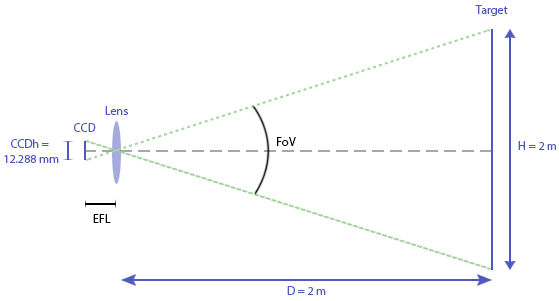
\includegraphics[scale=0.7]{fig/FOV.png}
  \caption{Field of View and Effective Focal Length}
  \label{fig:FOV}
\end{figure}

A simple relationship between the distance lens-target, the size of the target and the FoV can be deduced from the detailed diagram \ref{fig:FOV}: 
\begin{equation*}
tan( \frac{FoV}{2}) = \frac{1}{2} \times \frac{H}{D}
\end{equation*}
We derive and get
\begin{equation*}
 \frac{FoV}{2} = atan(\frac{1}{2} \times \frac{H}{D})
\end{equation*}

Numerically, with our problem delimitation, the Field of View is equal to $26.6\degree \times 26.6\degree$. 

\subsubsection{Focal Length}
\label{focalLength}
Thanks to the previous diagram, the Effective Focal Length (EFL) can also be determined: 
\begin{equation*}
EFL = \frac{1}{2} \times \frac{CCDh}{tan(\frac{FoV}{2})} = 12.29 \ mm
\end{equation*}
where $CCDh$ is the image section of the CCD according to the data sheet.\\

In order to get the real focal length, we choose $rf = 1 \ m$ for the distance of focus of the camera. 
\begin{equation*}
f = \frac{1}{\frac{1}{rf}+\frac{1}{EFL}} = 12.14 \ mm
\end{equation*}

\subsubsection{Aperture}
\label{aperture}
To determine the diameter of the aperture, several criteria have to be accounted for. If the diameter is too small, the sharpness of the image will decrease due to the diffraction effect. In fact, at large aperture, the diffracted light is negligible compared to the total amount of light entering the system. On the other hand, we should also consider the Depth of Field (FoV). We need to insure that it is big enough to allow us to see the whole target on the image. The relationship between the DoF and the diameter is inversely proportional. That means that if we increase the diameter, we will lessen it. The Diameter of Confusion (DoC), linked to the DoF is also a factor to take into consideration for the choice of the diameter. According to Wikipedia \cite{wiki:coc} It corresponds to \say{an optical spot caused by a cone of light rays from a lens not coming to a perfect focus when imaging a point source}. The smaller the DoC is, which corresponds to a better focus, the bigger is the DoF, and also the smaller is the diameter.

As the behaviour of the depth of field and of the diameter of confusion runs counter to the diffraction one, a trade-off has to be found. 

These formula are used to calculate the diameter of confusion and the diffraction spot:
\begin{equation*}
DoC = Dsr \cdot \frac{|r-rf|}{r} \cdot \frac{f}{rf - f}
\end{equation*}
where $Dsr$ is the diameter of the aperture
\begin{equation*}
DiffractionSpot = 2 \cdot EFL \cdot tan(1.22 \cdot \frac{lambda}{Dsr})
\end{equation*}
where $lambda$ is a wavelength of the sunlight\\

In the delimitations, it is assumed that the wavelengths of the sunlight belong to [400 800] nm. To settle on a diameter, the diameter of confusion and the diffraction spot were computed for diameters varying from 1 mm to 5 mm and wavelengths from 400 nm to 800 nm. The results are shown graphically in figure \ref{fig:DoCDifspot}. As the diameter of confusion cannot be bigger than the height of a pixel, the line corresponding to 12 $\mu m$ was also added to the graphic. In order to have the best trade-off, that is to say all the curves under 12 $\mu m$, we have chosen a effective lens entrance aperture $Dsr$ equal to $1.9 \ mm$, corresponding to $DoC = 0.0117 \ mm$. 

\begin{figure}[H]
  \centering
  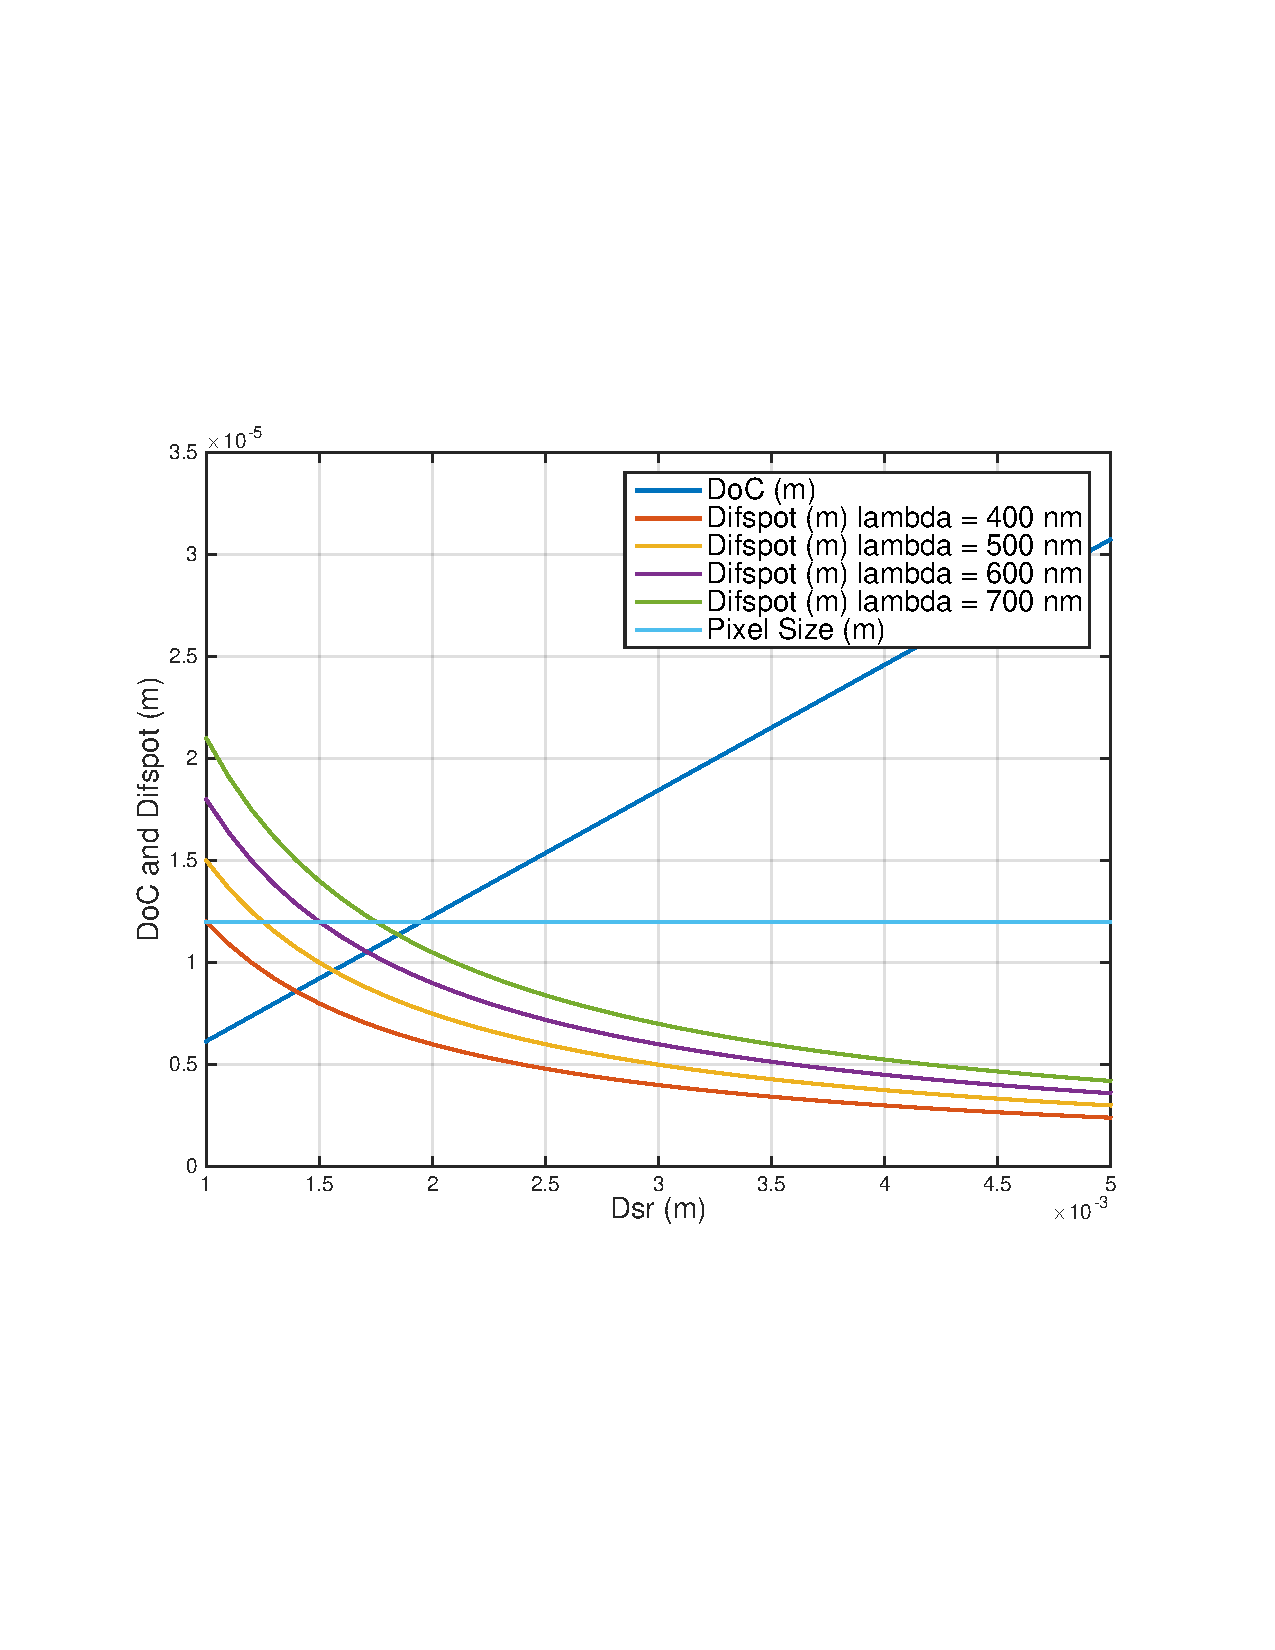
\includegraphics[trim=2cm 7cm 2cm 7cm, clip=true, totalheight=0.45\textheight, angle=0]{fig/DoCDifspot.pdf}
  \caption{Diameter of confusion and diffraction spots as a function of the diameter}
  \label{fig:DoCDifspot}
\end{figure}

Then, the depth of field can be deduced:
\begin{equation*}
DoF = \frac{2\frac{f}{Dsr}DoC(m+1)}{m^2 - (\frac{DoC}{Dsr})^2} = 1.33 \ m\\
where \ m = \frac{EFL}{rf} \ and \ is \ the \ magnification  
\end{equation*}
That means that the roughness of the rock analysed cannot be more than $\frac{DoF}{2} =  66.5\ cm$ since we could not see the whole rock if not, and the 3D map will then be flawed.